\documentclass[tikz,border=12pt]{standalone}
\usepackage[T1]{fontenc}
\usepackage{mathpazo}
\usepackage{amsmath,amssymb}
\usetikzlibrary{arrows.meta, positioning, calc, shapes.geometric}

\definecolor{stblue}{HTML}{7B97AD}
\definecolor{rwgold}{HTML}{B8995E}
\definecolor{sage}{HTML}{7A9A7E}
\definecolor{dkbrown}{HTML}{3D3530}
\definecolor{wmgray}{HTML}{7B7067}
\definecolor{cream}{HTML}{F9F6F0}
\definecolor{border}{HTML}{D4C9B8}

\begin{document}
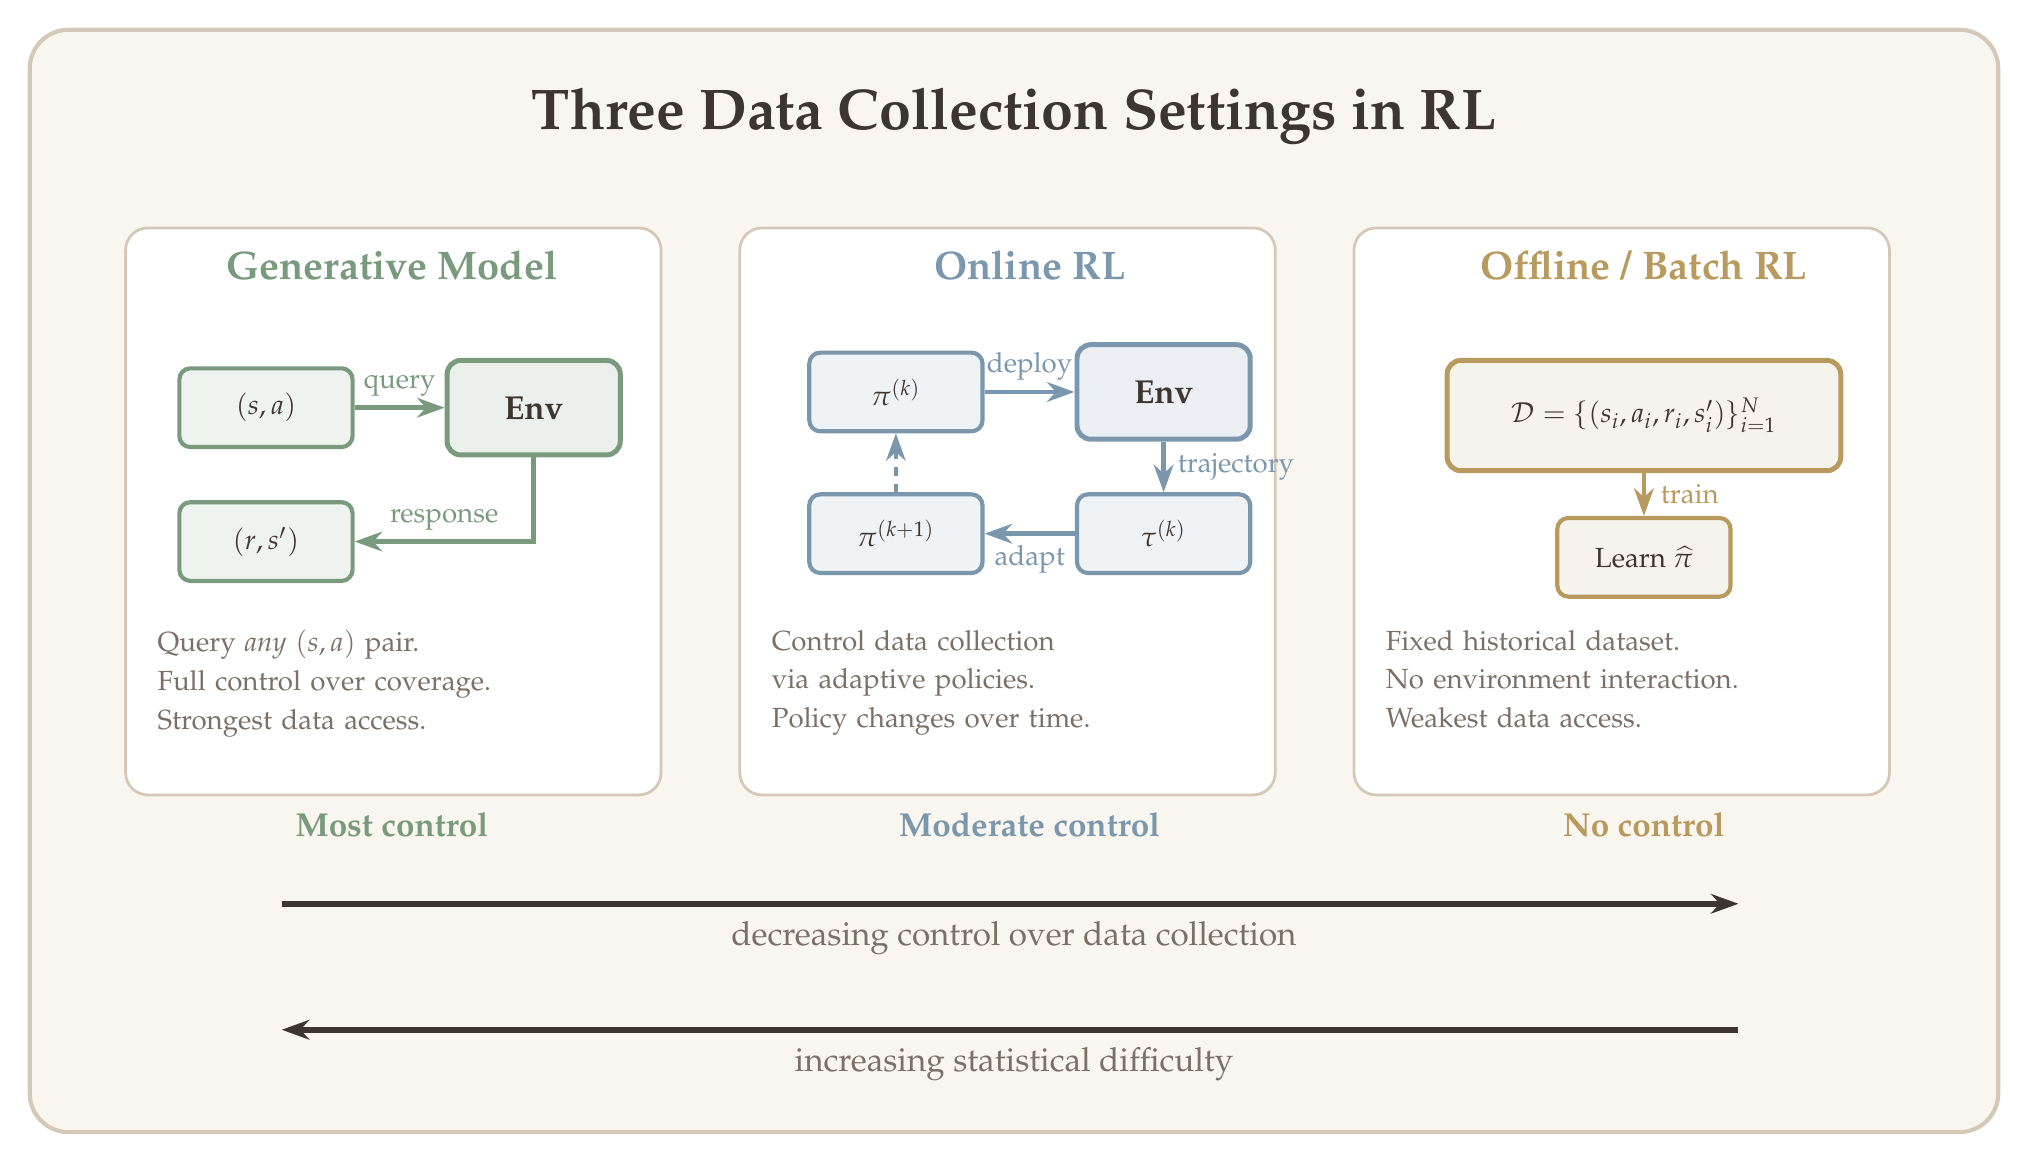
\begin{tikzpicture}[
  >={Stealth[length=3.5mm, width=2.5mm]},
  panel/.style={draw=border, line width=1pt, rounded corners=8pt, fill=white,
    minimum width=68mm, minimum height=72mm, anchor=north west},
  ptitle/.style={font=\Large\bfseries, text=dkbrown},
  desc/.style={font=\normalsize, text=wmgray, align=left, anchor=north west, text width=62mm},
  arr/.style={->, line width=1.4pt, dkbrown},
  sm/.style={draw=#1, line width=1.8pt, fill=#1!15, rounded corners=5pt,
    minimum width=22mm, minimum height=12mm, font=\large\bfseries, inner sep=3pt, text=dkbrown},
  sq/.style={draw=#1, line width=1.5pt, fill=#1!12, rounded corners=4pt,
    minimum width=22mm, minimum height=10mm, font=\normalsize, inner sep=3pt, text=dkbrown},
]

% Background
\fill[cream, rounded corners=14pt] (-1.2,-8.5) rectangle (23.8,5.5);
\draw[border, rounded corners=14pt, line width=1.5pt] (-1.2,-8.5) rectangle (23.8,5.5);

% Title
\node[font=\huge\bfseries, text=dkbrown] at (11.3,4.4)
  {Three Data Collection Settings in RL};

% === Panel 1: Generative Model ===
\node[panel] (p1) at (0.0,3.0) {};
\node[ptitle, text=sage] at (3.4,2.5) {Generative Model};

\node[sq=sage] (q1) at (1.8,0.7) {\textbf{$(s,a)$}};
\node[sm=sage] (env1) at (5.2,0.7) {Env};
\node[sq=sage] (o1) at (1.8,-1.0) {\textbf{$(r, s')$}};
\draw[arr, sage, line width=1.6pt] (q1) -- (env1) node[midway, above, font=\normalsize] {query};
\draw[arr, sage, line width=1.6pt] (env1) |- (o1) node[pos=0.75, above, font=\normalsize] {response};

\node[desc] at (0.3,-2.0) {Query \emph{any} $(s,a)$ pair.\\[2pt]
Full control over coverage.\\[2pt]
Strongest data access.};

\node[font=\large\bfseries, text=sage] at (3.4,-4.6) {Most control};

% === Panel 2: Online RL ===
\node[panel] (p2) at (7.8,3.0) {};
\node[ptitle, text=stblue] at (11.5,2.5) {Online RL};

\node[sq=stblue] (pi2) at (9.8,0.9) {$\pi^{(k)}$};
\node[sm=stblue] (env2) at (13.2,0.9) {Env};
\node[sq=stblue] (tau2) at (13.2,-0.9) {$\tau^{(k)}$};
\node[sq=stblue] (pi2next) at (9.8,-0.9) {$\pi^{(k+1)}$};

\draw[arr, stblue, line width=1.6pt] (pi2) -- (env2) node[midway, above, font=\normalsize] {deploy};
\draw[arr, stblue, line width=1.6pt] (env2) -- (tau2) node[midway, right=1pt, font=\normalsize] {trajectory};
\draw[arr, stblue, line width=1.6pt] (tau2) -- (pi2next) node[midway, below, font=\normalsize] {adapt};
\draw[arr, stblue, dashed, line width=1.2pt] (pi2next) -- (pi2);

\node[desc] at (8.1,-2.0) {Control data collection\\[2pt]
via adaptive policies.\\[2pt]
Policy changes over time.};

\node[font=\large\bfseries, text=stblue] at (11.5,-4.6) {Moderate control};

% === Panel 3: Offline / Batch RL ===
\node[panel] (p3) at (15.6,3.0) {};
\node[ptitle, text=rwgold] at (19.3,2.5) {Offline / Batch RL};

\node[draw=rwgold, line width=1.8pt, fill=rwgold!12, rounded corners=5pt,
  minimum width=50mm, minimum height=14mm, font=\normalsize, text=dkbrown,
  align=center] (data3) at (19.3,0.6)
  {$\mathcal{D} = \{(s_i, a_i, r_i, s_i')\}_{i=1}^N$};

\node[sq=rwgold] (learn3) at (19.3,-1.2) {Learn $\widehat{\pi}$};
\draw[arr, rwgold, line width=1.6pt] (data3) -- (learn3) node[midway, right=2pt, font=\normalsize] {train};

\node[desc] at (15.9,-2.0) {Fixed historical dataset.\\[2pt]
No environment interaction.\\[2pt]
Weakest data access.};

\node[font=\large\bfseries, text=rwgold] at (19.3,-4.6) {No control};

% === Bottom: control spectrum arrow ===
\draw[dkbrown, line width=2pt, ->] (2.0,-5.6) -- (20.5,-5.6);
\node[font=\large, text=wmgray, anchor=north] at (11.3,-5.7)
  {decreasing control over data collection};

% === Bottom: difficulty arrow ===
\draw[dkbrown, line width=2pt, <-] (2.0,-7.2) -- (20.5,-7.2);
\node[font=\large, text=wmgray, anchor=north] at (11.3,-7.3)
  {increasing statistical difficulty};

\end{tikzpicture}
\end{document}
